
% \documentclass{beamer}[10]
\documentclass[handout]{beamer}[10]
\usepackage{pgf}
\usepackage[danish]{babel}
\usepackage[utf8]{inputenc}
\usepackage{beamerthemesplit}
\usepackage{graphics,epsfig, subfigure}
\usepackage{url}
\usepackage{srcltx}
\usepackage{hyperref}
\usepackage{bookmark}
\usepackage{nicefrac}
\usepackage{multicol}
\usepackage{vwcol}
\usepackage{microtype}
\usepackage[all]{xy}
\usepackage{amssymb}


\definecolor{kugreen}{RGB}{50,93,61}
\definecolor{kugreenlys}{RGB}{132,158,139}
\definecolor{kugreenlyslys}{RGB}{173,190,177}
\definecolor{kugreenlyslyslys}{RGB}{214,223,216}
\setbeamercovered{invisible}
\mode<presentation>
\usetheme[numbers,totalnumber,compress,sidebarshades]{PaloAlto}
\setbeamertemplate{footline}[frame number]

  \usecolortheme[named=kugreen]{structure}
  \useinnertheme{circles}
  \usefonttheme[onlymath]{serif}
  \setbeamercovered{invisible}
  \setbeamertemplate{blocks}[rounded][shadow=true]

\logo{
\includegraphics[width=0.8cm]{KULogo}}
%\useoutertheme{infolines} 
\title{Equations in Hyperbolic(-esque) Groups}
\author{Barak Ohana}
\institute{The Hebrew University of Jerusalem}
\date{9 Sep 2024}

\newcommand{\sol}{\text{V}_{\Gamma}}
\renewcommand{\hom}{\text{Hom}}

%mathcal

\newcommand{\cala}{\mathcal{A}}
\newcommand{\calb}{\mathcal{B}}
\newcommand{\calc}{\mathcal{C}}
\newcommand{\cald}{\mathcal{D}}
\newcommand{\cale}{\mathcal{E}}
\newcommand{\calf}{\mathcal{F}}
\newcommand{\calg}{\mathcal{G}}
\newcommand{\calh}{\mathcal{H}}
\newcommand{\cali}{\mathcal{I}}
\newcommand{\calj}{\mathcal{J}}
\newcommand{\calk}{\mathcal{K}}
\newcommand{\call}{\mathcal{L}}
\newcommand{\calm}{\mathcal{M}}
\newcommand{\caln}{\mathcal{N}}
\newcommand{\calo}{\mathcal{O}}
\newcommand{\calp}{\mathcal{P}}
\newcommand{\calq}{\mathcal{Q}}
\newcommand{\calr}{\mathcal{R}}
\newcommand{\cals}{\mathcal{S}}
\newcommand{\calt}{\mathcal{T}}
\newcommand{\calu}{\mathcal{U}}
\newcommand{\calv}{\mathcal{V}}
\newcommand{\calw}{\mathcal{W}}
\newcommand{\calx}{\mathcal{X}}
\newcommand{\caly}{\mathcal{Y}}
\newcommand{\calz}{\mathcal{Z}}

%mathbb
\usepackage{amsfonts}
\renewcommand{\aa}{\mathbb{A}}
\newcommand{\bb}{\mathbb{B}}
\newcommand{\cc}{\mathbb{C}}
\newcommand{\dd}{\mathbb{D}}
\newcommand{\ee}{\mathbb{E}}
\newcommand{\ff}{\mathbb{F}}
\renewcommand{\gg}{\mathbb{G}}
\newcommand{\hh}{\mathbb{H}}
\newcommand{\ii}{\mathbb{I}}
\newcommand{\jj}{\mathbb{J}}
\newcommand{\kk}{\mathbb{K}}
\renewcommand{\ll}{\mathbb{L}}
\newcommand{\mm}{\mathbb{M}}
\newcommand{\nn}{\mathbb{N}}
\newcommand{\oo}{\mathbb{O}}
\newcommand{\pp}{\mathbb{P}}
\newcommand{\qq}{\mathbb{Q}}
\newcommand{\rr}{\mathbb{R}}
\renewcommand{\ss}{\mathbb{S}}
\renewcommand{\tt}{\mathbb{T}}
\newcommand{\uu}{\mathbb{U}}
\newcommand{\vv}{\mathbb{V}}
\newcommand{\ww}{\mathbb{W}}
\newcommand{\xx}{\mathbb{X}}
\newcommand{\yy}{\mathbb{Y}}
\newcommand{\zz}{\mathbb{Z}}

%parentheses
\newcommand*{\rb}[1]{\left( #1 \right)}
\renewcommand*{\sb}[1]{\left[ #1 \right]}
\newcommand*{\cb}[1]{\left\{ #1 \right\}}
\newcommand*{\ab}[1]{\left< #1 \right>}
\newcommand*{\nb}[1]{\lVert #1 \rVert}
\newcommand{\size}[1]{\left| #1 \right|}

\newcommand*{\by}{\pmb{Y}}
\DeclareMathOperator{\diam}{diam}
\DeclareMathOperator{\mcg}{MCG}
\newcommand{\sker}{\underset{\rightarrow}{\ker}}
\newcommand{\onto}{\twoheadrightarrow}
\DeclareMathOperator{\cay}{Cay}
\newcommand{\acts}{\curvearrowright}

\graphicspath{ {images/} }



\begin{document}
\begin{frame}\titlepage \vspace{-0.5cm}\end{frame}


\section{First section}

\begin{frame}
    \frametitle{Equations in Groups}
    \pause
    Let $\Gamma$  be a group,\pause and let $\Sigma\left(x_{1},\ldots,x_{d}\right)$ a (possibly infinite) system of equation on d variables. \pause
    We define the \textbf{set of solution of $\Sigma$ in $\Gamma$} to be the set
    \begin{equation*}
        \sol\left(\Sigma\right)=\left\{ \left(g_{1},\ldots,g_{d}\right)\in\Gamma^{d}\mid\Sigma\left(g_{1},\ldots,g_{d}\right)=_{\Gamma}1\right\} 
    \end{equation*}

            \pause

    There is an equivalence
    \begin{equation*}
        \sol\rb{\Sigma} \leftrightarrow \hom\rb{\nicefrac{\ff_d}{\ab{\ab{\Sigma}}}, \Gamma}
    \end{equation*}

    \pause

    So instead of studying solutions in $\Gamma$ we will study homomorphisms to $\Gamma$.

\end{frame}


\subsection{Sample subsection}

\begin{frame}

\frametitle{Sample Frame Title No. 2}

\begin{definition}
    A group $\Gamma$ is called equationally noetherian if  every set of equation is equivalent to a finite subset of it. \pause i.e. if for any set of equation $\Sigma$ there exists a finite subset $\Sigma_0$ such that $\sol\rb{\Sigma} = \sol\rb{\Sigma_0}$.
\end{definition}
\pause
\begin{example}\pause
    \begin{multicols}{2}
    \begin{itemize}
        \item All finite Groups \pause
        \item All linear groups\pause
            \begin{itemize}
                \item Thus all free groups\pause
            \end{itemize}
        \item Hyperbolic groups\\\pause
        \item[] 
        \item Free product of equationally noetherian groups\pause
        \item Groups hyperbolic relative to equationally noetherian
    \end{itemize}
    \end{multicols}
\end{example}

\end{frame}

\section{Limit groups}



\begin{frame}
    \frametitle{Limit group}
\pause 
    \begin{definition}\pause
        Let $\Gamma$ be a f.g. \pause  and $\rb{\varphi_n} \in \hom\rb{G,\Gamma}$ for some f.g. group $G$. \pause
        We define the \textbf{stable kernel} of $\rb{\varphi_n}$ to be
        \begin{equation*}
            \sker{\varphi_n} = \cb{g\in G \mid \varphi_n \rb{g} \text{is eventually } 1}
        \end{equation*}
        And e define the corrsponding \textbf{limit group} by $L=\nicefrac{G}{\sker{\varphi_n}}$
    \end{definition}
    \pause
    \begin{lemma}
        Let $\Gamma$ be a group then the following are equivalent:

        \begin{itemize}
            \item $\Gamma$ is equationally noetherian
            \pause \item For any f.g. $G$ and any $\rb{\varphi_n} \in \hom\rb{G,\Gamma}$, \pause $\varphi_n$ eventually factors through the
            quotient $G\onto L$
        \end{itemize}

    \end{lemma}
\end{frame}

\begin{frame}
    \begin{block}{Reminder}
        $\rb{\varphi_n} \in \hom\rb{G,\Gamma}$ factors through $G\onto L$ if and only if $\sker\rb{\varphi_n} \subseteq \ker \varphi_n $. 
        
        Thus we want to show that we have that eventually we have $\sker\rb{\varphi_n} \subseteq \ker \varphi_n $.
    \end{block}
\end{frame}

\begin{frame}

    Let $\Gamma$ be a f.g. hypebolic group, meaning its caylel graph is hyperbolic.
    
    \pause Let $\rb{\varphi_n} \in \hom\rb{G,\Gamma}$. 
    
    \pause We want to show that $\varphi_n$ eventually factors through $L$.
    
    \pause Denote 
    \begin{equation*}
        \nb{\varphi_n} = \max_{s\in S} d_\Gamma \rb{1,\varphi_n\rb{ s }}
    \end{equation*}\pause
    i.e. the maximal lenght of the images of the generators of $G$ under $\varphi_n$.\pause
    \begin{fact}
        If $\nb{\varphi_n}$ is a bounded sequence then $\varphi_n$ has finitely many options (as morphisms).
        
        Thus if $\nb{\varphi_n}$ is a bounded sequence then $\varphi_n$ eventually factors through $G\onto L$.
    \end{fact}

\end{frame}

% \begin{frame}
%     Assume that $\nb{\varphi_n}$ is not bounded.
%     Define at the sequence of matric spaces 
%     \begin{equation*}
%         X_n = \frac{1}{\nb{\varphi_n}} \cay \rb{ \Gamma } \pause  ; d_n \rb{ x,y }=\frac{1}{\nb{\varphi_n}} d_{\cay \rb{ \Gamma }} \rb{x,y}
%     \end{equation*}
%     \pause The rescaling of the cayley graph of $\Gamma$. \pause Now one can look at the asymptotic cone of the $X_n$'s \pause
%     \begin{equation*}
%                 T=\lim X_n = \nicefrac{\cb{\sb{x_n} \mid x_n\in X_n}}{\ab{\sb{x_n}\sim\sb{y_n} \iff \lim d_n \rb{x_n,y_n} = 0}}
%     \end{equation*}

%     This is a $\rr$-tree (here we used the hyperbolicity of $\cay\rb{\Gamma}$).
%     The group $G$ has an action on $T$, and since we took equivalence classes, also $L$ acts on $T$.

% \end{frame}

% \begin{frame}
%     We now call Sela and Rips, who tell us that the action $L \acts T$ means that $L$ is finitely presented relative to finitely many finitely generated subgroups $P_1,\ldots,P_d$ that fix a point in $T$.

%     \begin{block}{Observation}
%         If one shows that $\varphi_n\big\vert_{\tilde{P_i} }: \tilde{P_i} \to \Gamma$ (eventually) factors through $\tilde{P_i} \onto P_i$ then $\varphi_n$ eventually factors through $G\onto L$
%     \end{block}
% \end{frame}


% \begin{frame}
%     Let $P$ one of the subgroups of $L$ that fixes a point in $T$.

%     Why does $P$ fixes a point in $T$?
    
    

%     \begin{equation*}
%         \xymatrix{
%             G\ar@{->>}[d]\ar@/^/[ddr]^{\varphi_{n}} &           \\
%             P\leq L\hspace{5ex}                                       &           \\
%                                                     & \Gamma  
%         }\pause \hspace{8ex}
%         \begin{matrix}
%         \vspace{8ex}    \\
%         \rightsquigarrow \\
        
%         \end{matrix}
%         \hspace{8ex}
%         \xymatrix{
%             \tilde{P}\ar@{->>}[d]\ar@/^/[ddr]^{\varphi_{n}\big\vert_{\tilde{P}}}    &        \\
%             P                                                                       &        \\
%                                                                                     & \Gamma            
%         } 
%     \end{equation*}
% \end{frame}

% \begin{frame}
%     \frametitle{<title>}

%     \begin{itemize}
%         \item Option 1: $\nb{\varphi_{n}\big\vert_{\tilde{P}}}$ is bounded. In this case $$\varphi_{n}\big\vert_{\tilde{P}}$$ does factors through $G \onto L$
%         \item Option 2: $\nb{\varphi_{n}\big\vert_{\tilde{P}}}$ is unbounded, but much smaller (asymptotically) then $\nb{\varphi_{n}}$. 
        


%         We "scaled down" all the action of $\tilde{P}$ on $\cay{\Gamma}$



%     \end{itemize} 

%     In option 2 we define 
%     \begin{equation*}
%         X_{n}^{P} = \frac{1}{\nb{\varphi_{n}\big\vert_{\tilde{P}}}} \cay \rb{ \Gamma }
%     \end{equation*}
%     \begin{equation*}
%         T^{P}=\lim X_{n}^{\tilde{P}} = \nicefrac{\cb{\sb{x_n} \mid x_n\in X_{n}^{P}}}{\ab{\sb{x_n}\sim\sb{y_n} \iff \lim d_n \rb{x_n,y_n} = 0}}
%     \end{equation*} 

% \end{frame}

% \begin{frame}
%     \begin{equation*}
%         \begin{matrix}
%             \text{We now have} \\
%             P\acts T^p
%         \end{matrix}
%               \Longrightarrow  
%         \begin{matrix} 
%                 \text{$P$ is finitely presented relative to} \\
%                 \text{finitely many finitely generated subgroups} \\
%                 \text{$Q_1,\ldots,Q_d$ that fix a point in $T^P$}
%         \end{matrix}  
%     \end{equation*}

%     % \begin{center}
%         \begin{figure}
%             \begin{overprint}
%                 \onslide<1>\centering
\includegraphics[scale=0.2]{Step0.PNG}
%                 \onslide<2>\centering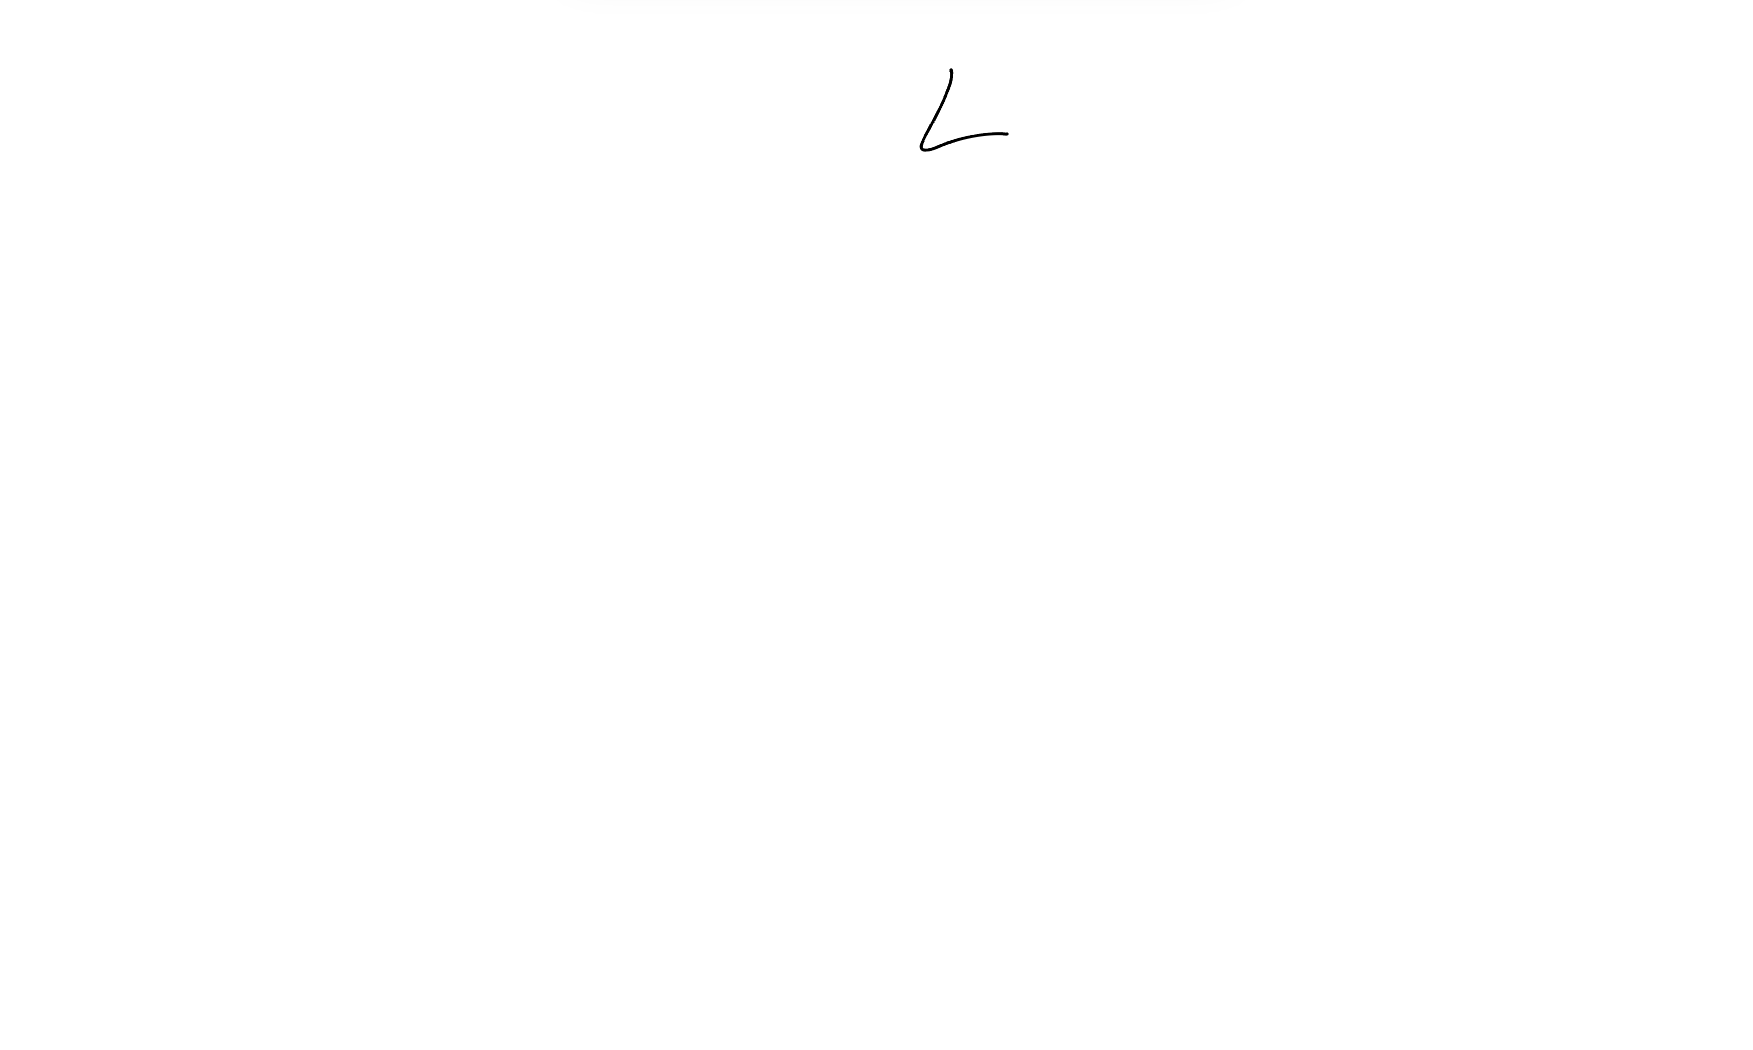
\includegraphics[scale=0.2]{Step1.PNG}
%                 \onslide<3>\centering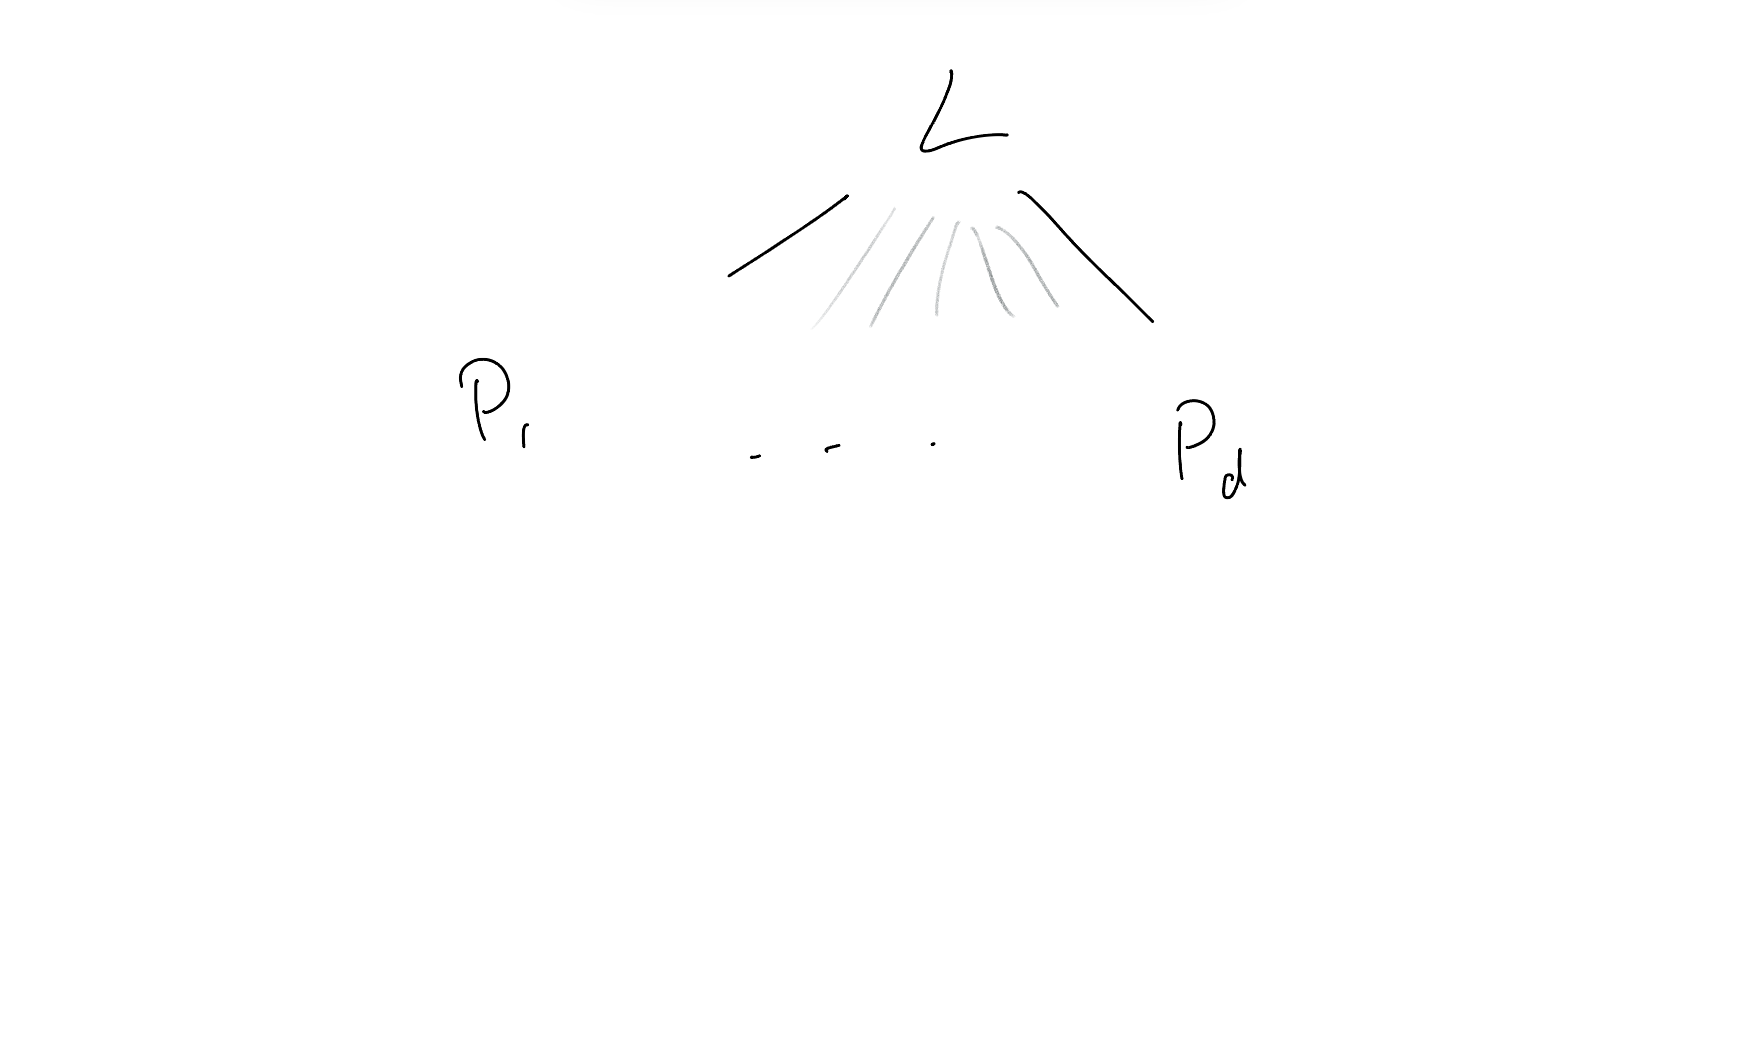
\includegraphics[scale=0.2]{Step2.PNG}
%                 \onslide<4>\centering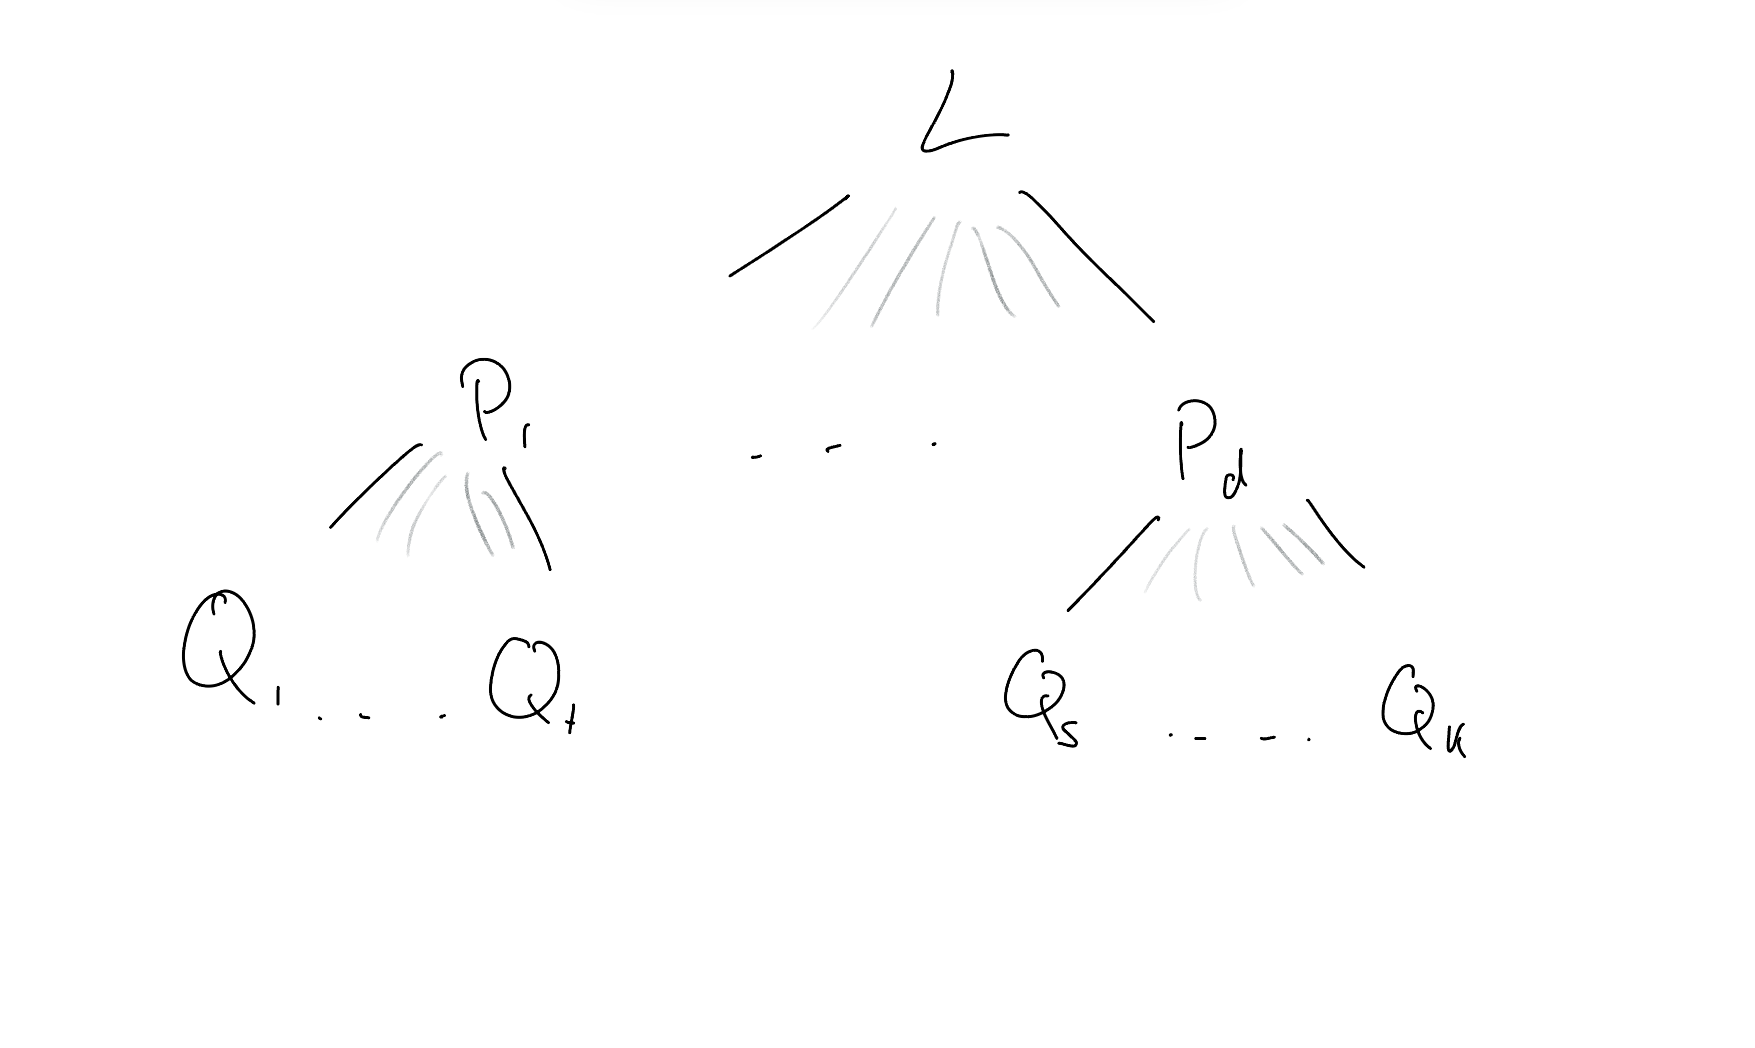
\includegraphics[scale=0.2]{Step3.PNG}
%                 \onslide<5>\centering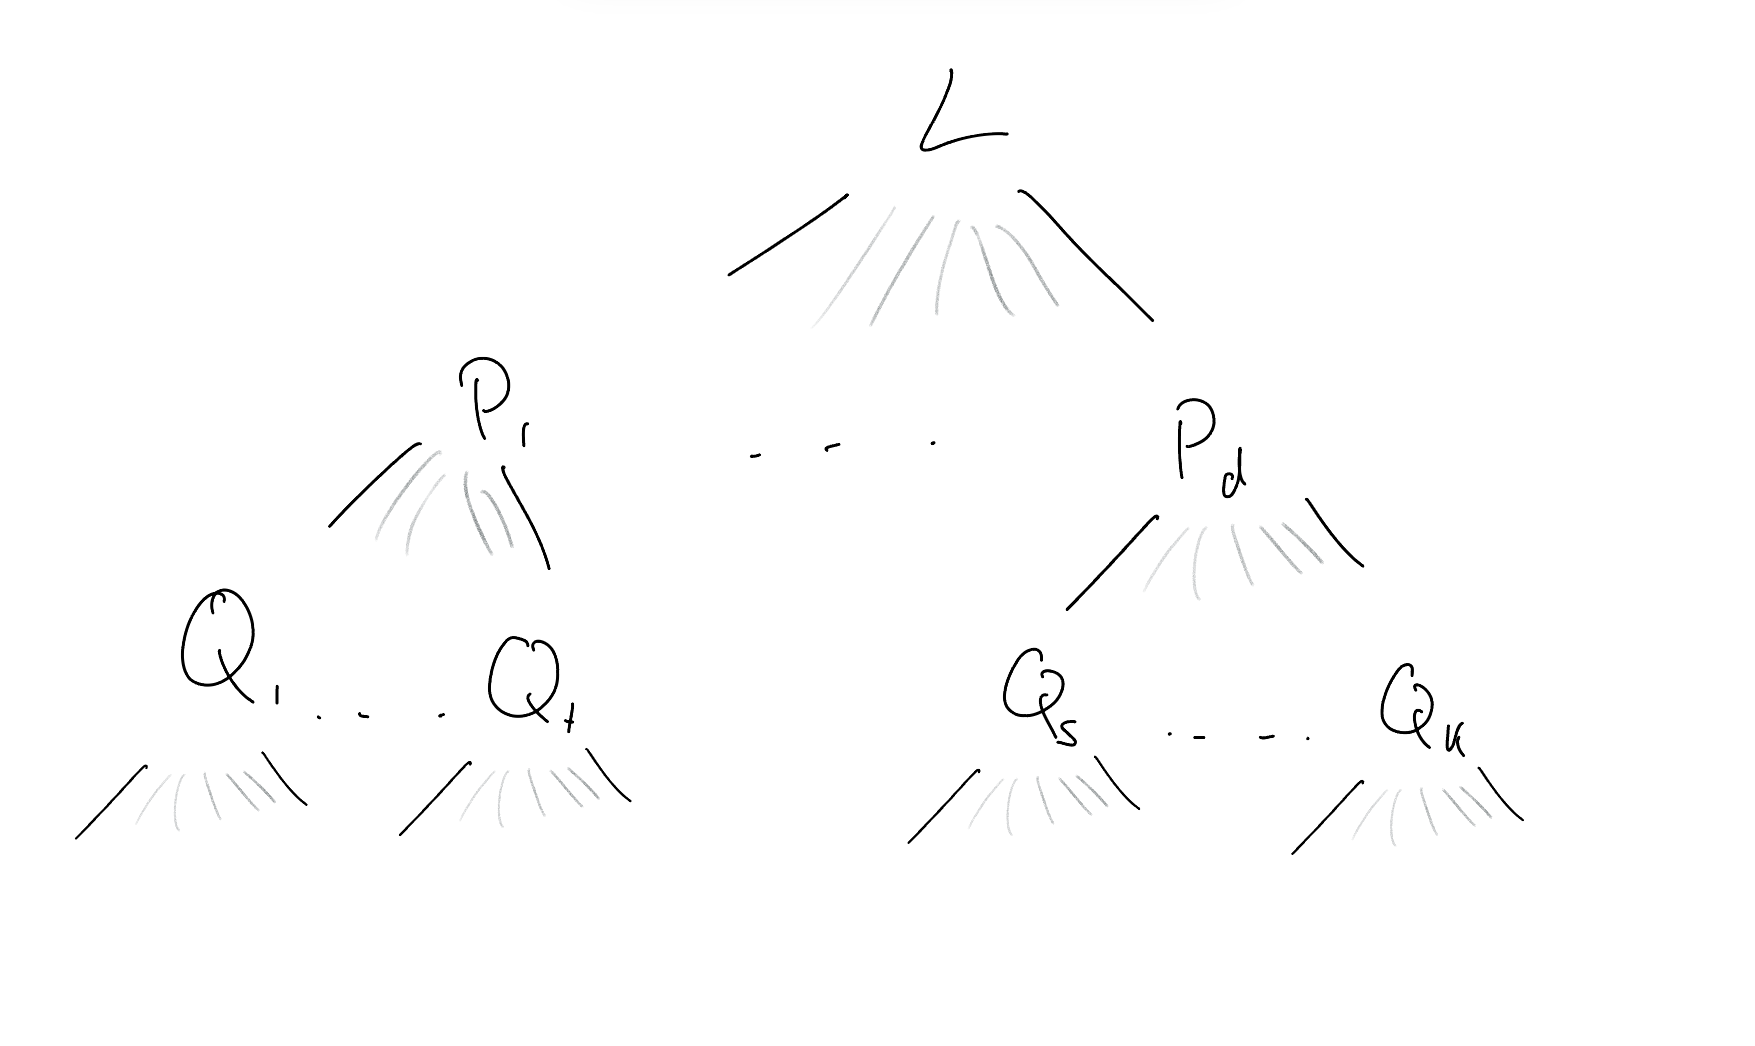
\includegraphics[scale=0.2]{Step4.PNG}
%                 \onslide<6->\centering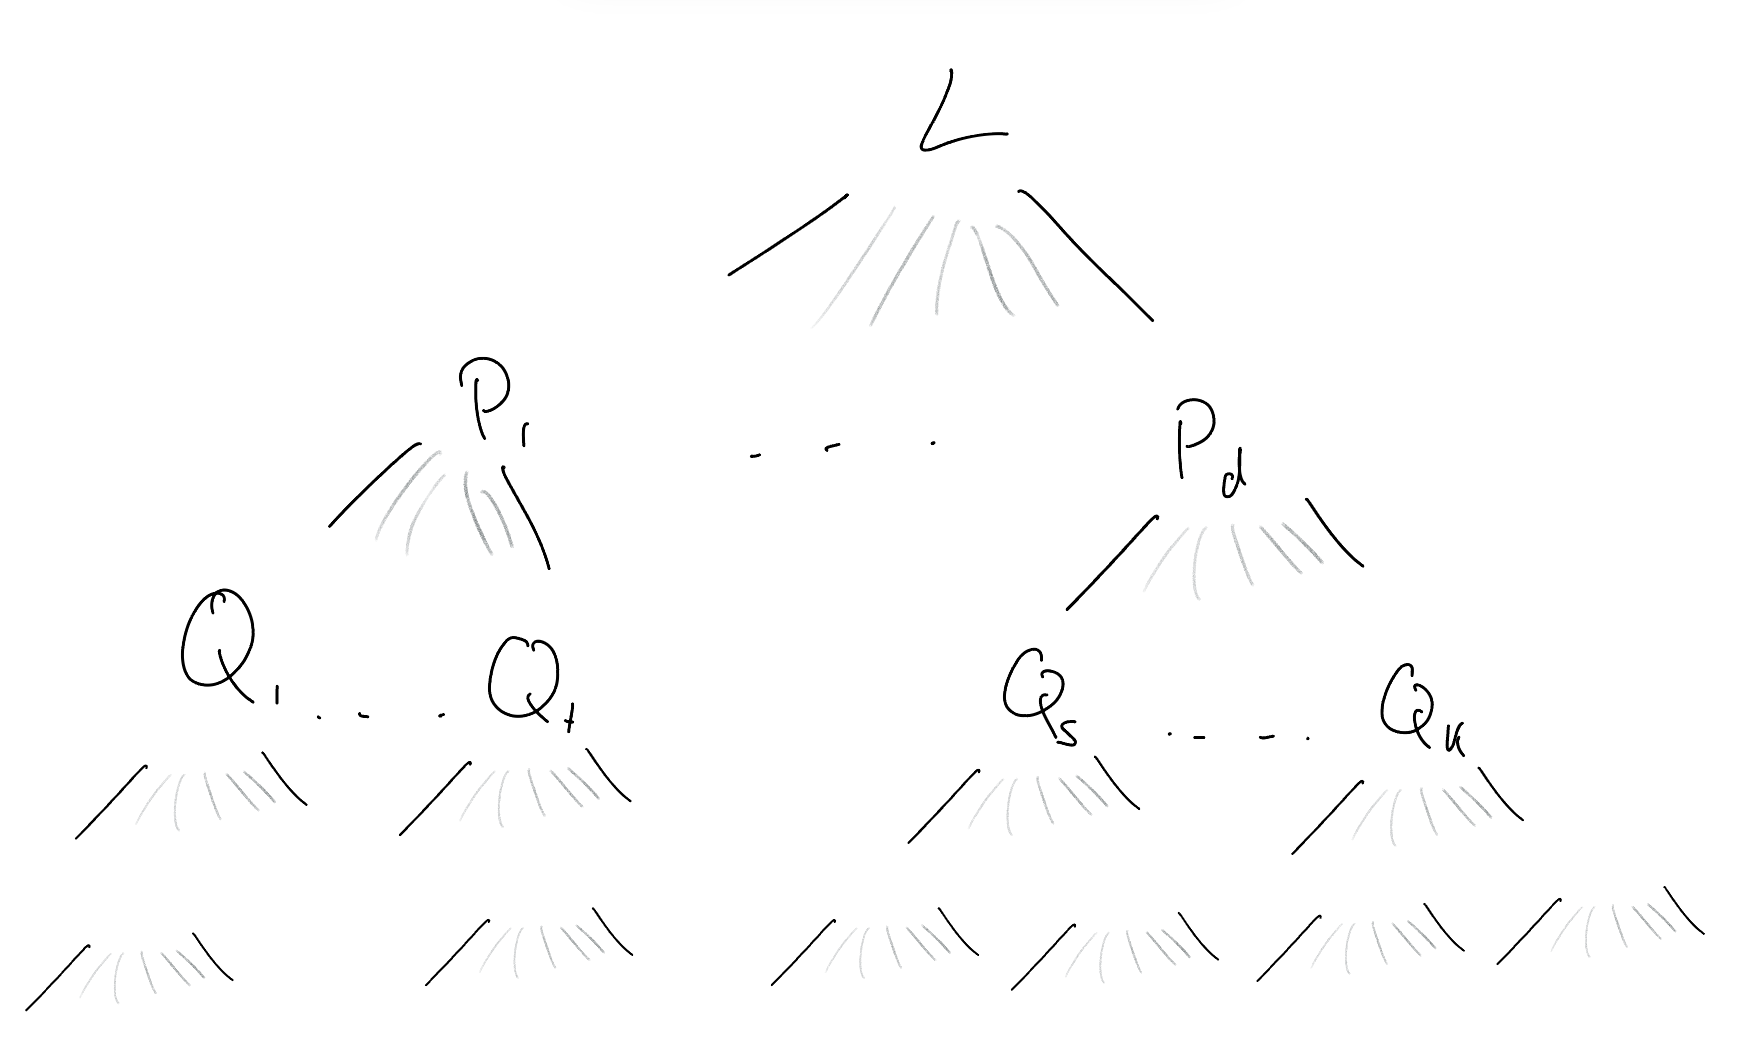
\includegraphics[scale=0.2]{Step5.PNG}
%             \end{overprint}
%         \end{figure}
%         % \includegraphics[scale=0.2]{./Shortening.png}
%     % \end{center}
% \end{frame}

\begin{frame}
    \begin{block}{Theorem (Sela, Weidmann-Reinfeldt)}
        $L$ is finitely presented relative to finitely many finitely generated subgroups $P_1, \ldots, P_d$ such that $\nb{\varphi_{n}\big\vert_{\tilde{P}_i}}$ is bounded for every $i$.

        Thus $\varphi_n$ eventually factors through $G \onto L$
    \end{block}

    Finitely presented relative to $P_1, \ldots, P_d$ means that
    \begin{equation*}
        L = \ab{ P_1, \ldots, P_d, S \mid R} 
    \end{equation*}
    where $S$ is a finite set of (extra) generators, and $R$ is a finite set of (extra) relations.

    \pause We have that $\varphi_n$ eventually factors through $G\onto L$ if and only if $\varphi_{n}\big\vert_{\tilde{P}_i}$ eventually factors through $\tilde{P}_i \onto P_i$

    
    \pause But $\nb{\varphi_{n}\big\vert_{\tilde{P}_i}}$ is bounded for every $i$, meaning that $\varphi_{n}\big\vert_{\tilde{P}_i} : \tilde{P}_i \to \Gamma$ factors through $\tilde{P}_i\to P_i$

\end{frame}

\begin{frame}
    \begin{block}{Theorem(Sela: torsion free hyp. groups, Weidmann-Reinfeldt: all hyp. groups)}
        If $\Gamma$ is a finitely generated hyperbolic group then $\Gamma$ is equationally noetherian.
    \end{block}
    \vspace*{4ex}
    But what happens with groups that are not hyperbolic?
\end{frame}

\begin{frame}
    \frametitle{Hyperbolic-esque Groups}
    Let $\Gamma$ be a finitely generated group acting on hyperbolic space $X$. Under some assumption on the actions, the same lemma apply

    \begin{block}{Theorem (Groves \& Hull, 2017)}
        Let $\Gamma$ be a group action acylidrically on a hyperbolic space $X$. Let $L$ be a limit group. \\
        
        $L$ is finitely presented relative to finitely many finitely generated subgroups $P_1, \ldots, P_d$ such that $\nb{\varphi_{n}\big\vert_{\tilde{P}_i}}$ is bounded for every $i$.

        Thus $\varphi_n$ eventually factors through $G \onto L$
    \end{block}



    Since $X$ is not the cayley graph we dont know that if $\nb{\varphi_n}$ is bounded then $\varphi_n$ eventually factors through $G\onto L$.
\end{frame}

\begin{frame}
    Let $\Gamma$ be a group acting acylidrically on two hyperbolic metric spaces, $X_1$ and $X_2$, such that $\Gamma \acts X_1 \times X_2$ is "like" the actions of $\Gamma$ on $\cay\rb{\Gamma}$.

    Let $P_1, \ldots, P_d$ be the groups from the lemma before, i.e. $L$ is f.p. relative to $P_1, \ldots, P_d$ and $\nb{\varphi_{n}\big\vert_{\tilde{P}_i}}_{X_1}$ (mesured in $X_1$!) is bounded.

    \vspace{2ex}

    We will explain why $\varphi_{n}\big\vert_{\tilde{P}_i}$ factors through $\tilde{P}_i \onto P_i$. 
\end{frame}


\begin{frame}
    Look at the group $\tilde{P}_i \leq G$. The Lemma before tels us that $P_i$ is finitely presented relative to $Q_1, \ldots, Q_l$ where
    \begin{equation*}
        \nb{\varphi_{n}\big\vert_{\tilde{Q}_j}}_{X_2}
    \end{equation*}

    Now mesured relative to $X_2$!
    Since $\tilde{Q}_l$ is a subgroup of $P_i$, then 
    \begin{equation*}
        \nb{\varphi_{n}\big\vert_{\tilde{Q}_j}}_{X_1 \times X_2} = \max_{s\in S} d_{X_1 \times X_2} \rb{1, \varphi_n \rb{s}}
    \end{equation*} 

    is bounded!

    Which means the $\varphi_{n}\big\vert_{\tilde{Q}_j}$ eventually factors through $\tilde{Q}_j \onto Q_j$. 

    Since this is true for all $Q_1, \ldots, Q_l$, then, as before, $\varphi_{n}\big\vert_{\tilde{P}_i}$ factors through $\tilde{P}_i \onto P_i$.

\end{frame}

\begin{frame}
    Now since $L$ is finitely presented relative to $P_1, \ldots ,P_d$ then $\varphi_n$ eventually factors through $G\onto L$.

    \begin{block}{Theorem (O')}
        Every f.g. group acting  geometrically and strictly acylindrically (i.e as before) on a product of hyperbolic spaces is equationally noetherian.
    \end{block}

    This method generalize to groups acting on colorable Hierarchically Hyperbolic spaces (whatever this means)
    \begin{block}{Theorem (O')}
        Every f.g. group acting strictly acylindrical on a colorable HHG is equationally noetherian.
    \end{block}


\end{frame}



\end{document}